\documentclass[Bachelorarbeit.tex]{subfiles}
\begin{document}

\graphicspath{{./figures/newMarket/}}	%specifying the folder for the figures

\chapter{A new Market}
In the thesis-software it is possible to run an ascending-connected topology until no more trades are possible and then activate the new market. the collateralized assets are bought and sold by the pessimists and move up the optimism-scale until they end up in the optimists.


neuer markt: Collateralisierte ASsets gegen Cash			
	Neuer Markt: Collateralisierte Assets gegen Cash
	Käufer: 		bekommt Asset und Loan, zahlt Cash
	Verkäufer: 		bekommt Cash und gibt Asset und Loan
	limit-preis für diesen markt?
	Fläche unter P/M/O gleich bei Fully-Connected und Ascending-Connected obwohl unterschiedliche

Erweiterung mit zweiter Hypothese
zweite Hypothese: erreicht ascending-connected nun mit dem neuen markt das gleichgewicht?
ergebnis der zweiten hypothese: funktioniert
		
\section{Results with the new market}	
As experiment-configuration the same as given in Chapter 5 "Results" is used.

\begin{table}[h]
	\centering
	\caption{Configuration for all experiments}
	\begin{tabular} { l c r }
		\hline
		Agent-Count & 100 \\
		Bond-Type & 0.5 \\
		Replication-Count & 50 \\
		Terminate after & 1000 failed successive Transactions \\
		\hline
	\end{tabular}
\end{table}

\subsection{Fully-Connected}
\begin{figure}[H]
	\centering
  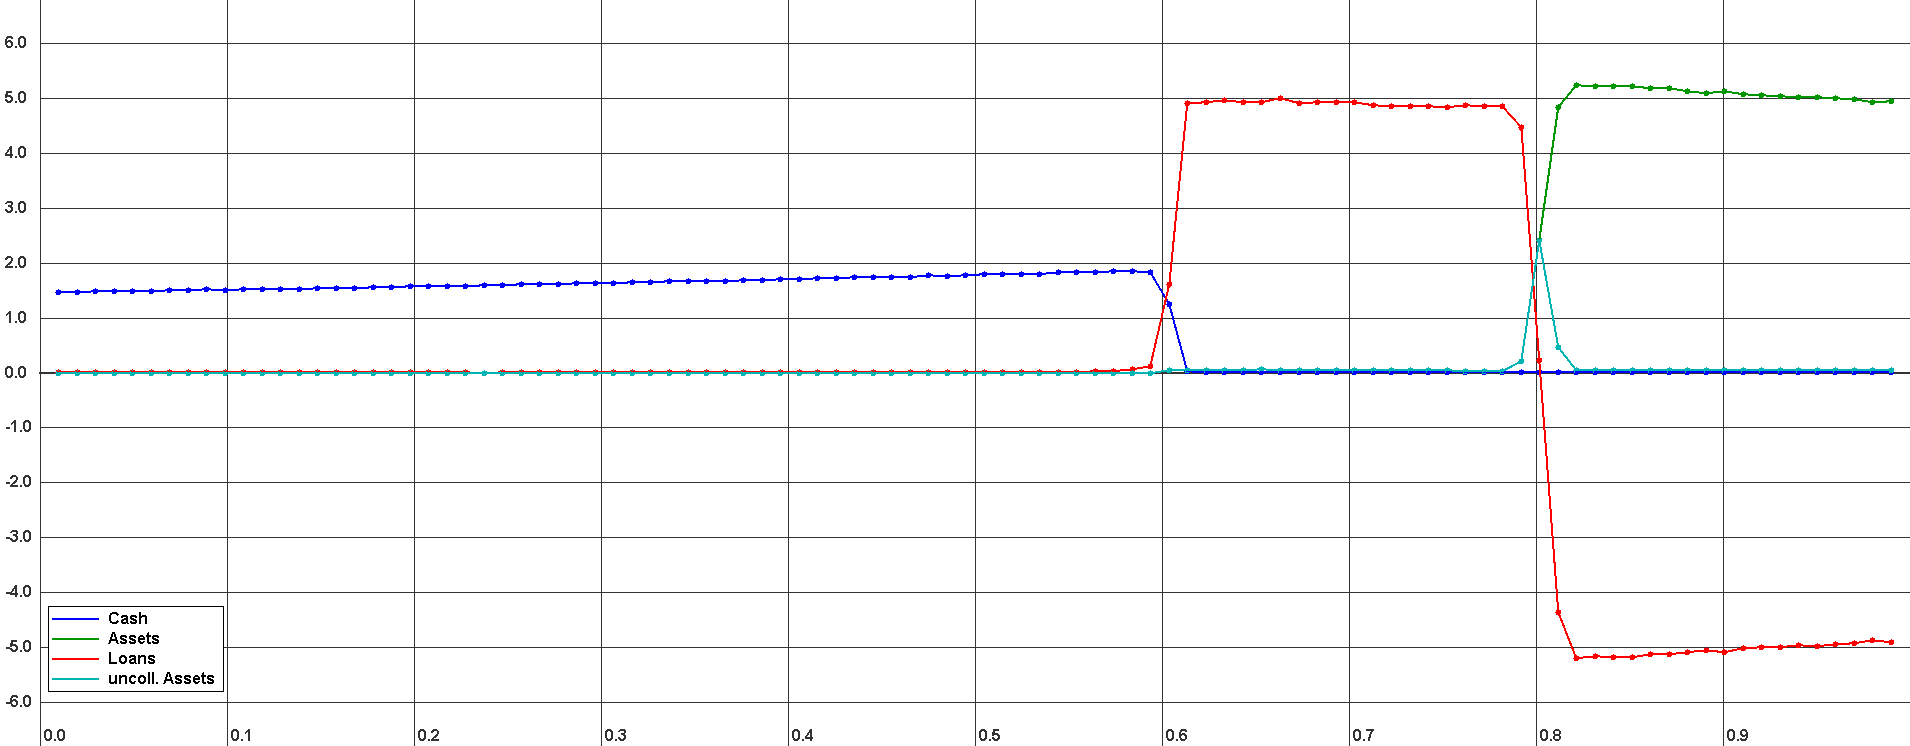
\includegraphics[width=1.0\textwidth, angle=0]{FULLYCONNECTED_100_WITHCOLLATERALMARKET_REPL.png}
	\caption{Wealth-Distribution of Fully-Connected topology}
	\label{fig:wealth_FULLYCONNECTED_100_WITHCOLLATERALMARKET_REPL}
\end{figure}

\begin{figure}[H]
	\centering
  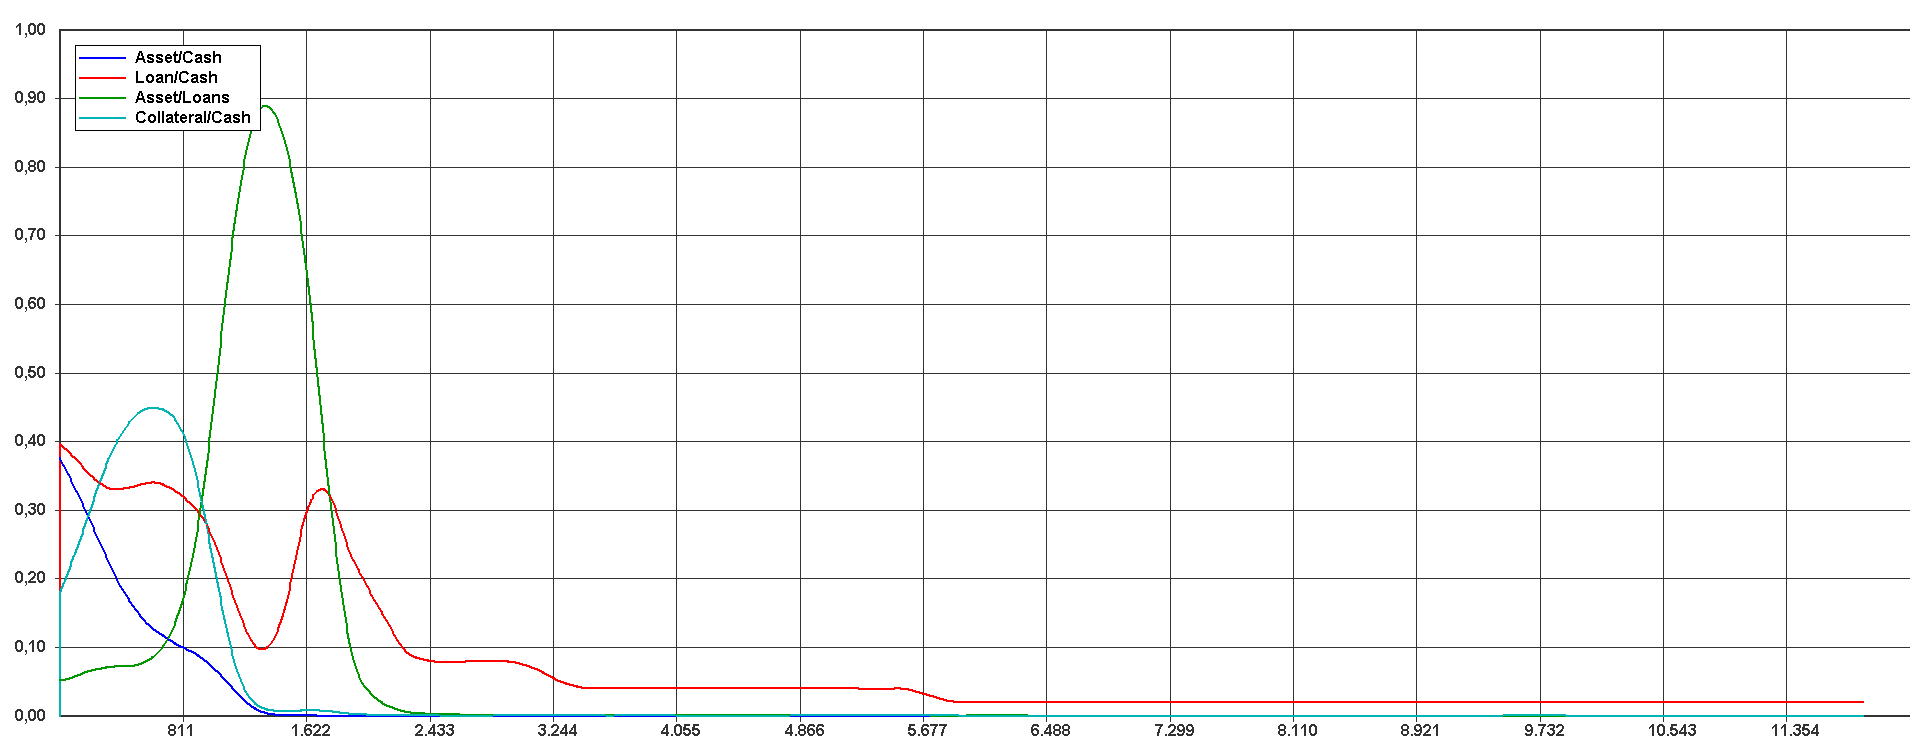
\includegraphics[width=1.0\textwidth, angle=0]{FULLYCONNECTED_100_WITHCOLLATERALMARKET_MARKETSTIME_REPL.png}
  	\caption{Market-activity over time of Fully-Connected topology}
	\label{fig:wealth_FULLYCONNECTED_100_WITHCOLLATERALMARKET_MARKETSTIME_REPL}
\end{figure}

\begin{figure}[H]
	\centering
  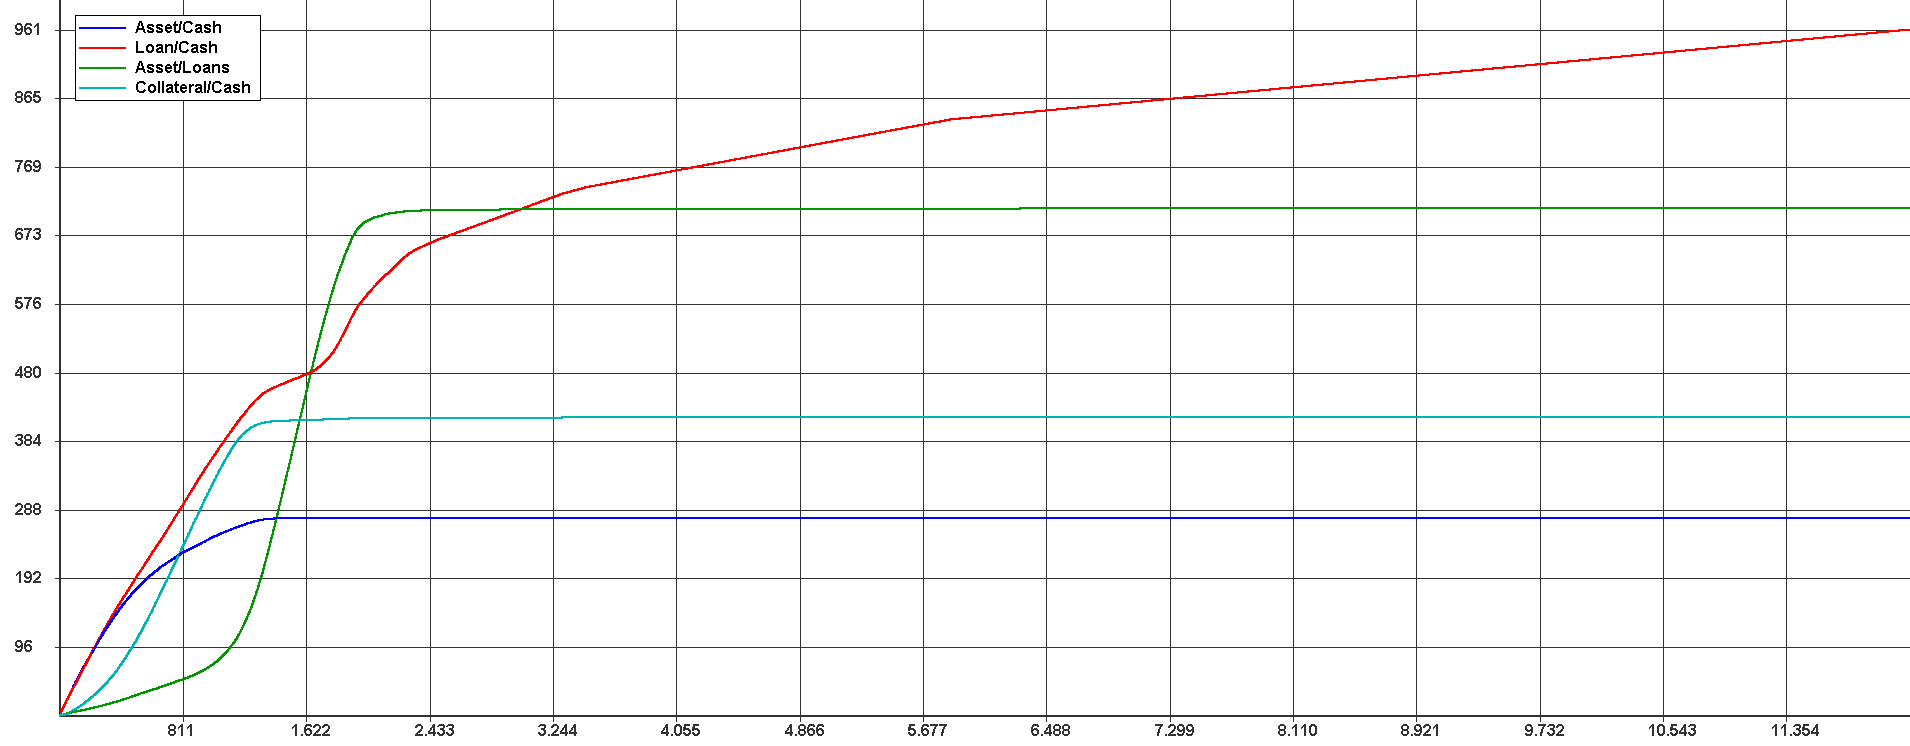
\includegraphics[width=1.0\textwidth, angle=0]{FULLYCONNECTED_100_WITHCOLLATERALMARKET_MARKETSACCUM_REPL.png}
	\caption{Market-activity accumulated of Fully-Connected topology}
	\label{fig:wealth_FULLYCONNECTED_100_WITHCOLLATERALMARKET_MARKETSACCUM_REPL}
\end{figure}

\subsection{Ascending-Connected}
\begin{figure}[H]
	\centering
  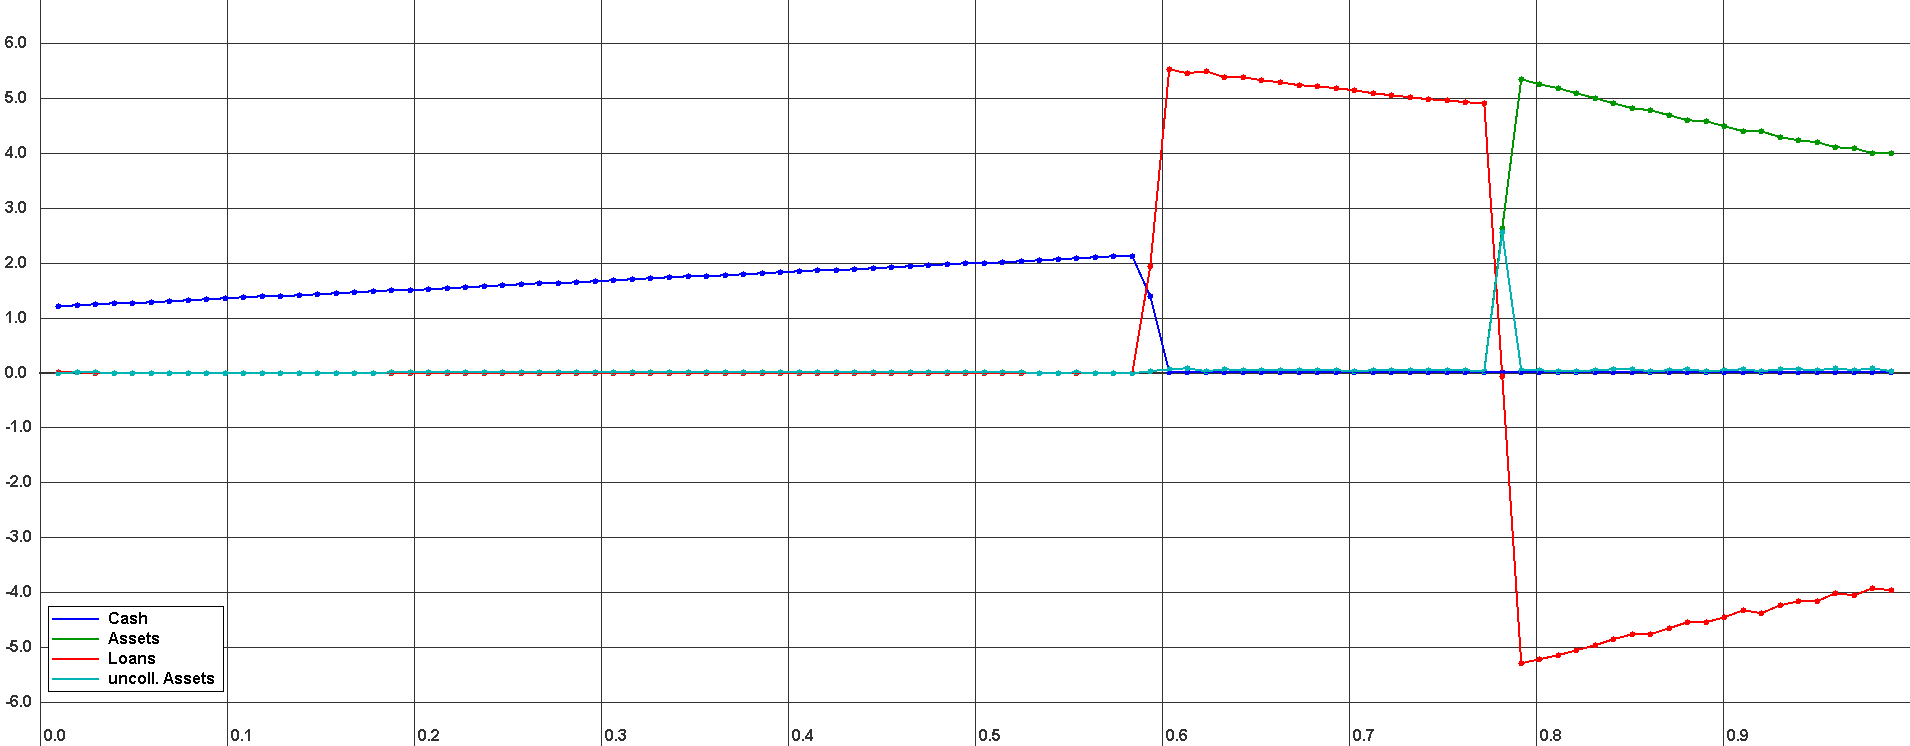
\includegraphics[width=1.0\textwidth, angle=0]{ASCENDINGCONNECTED_100_WITHCOLLATERALMARKET_REPL.png}
	\caption{Wealth-Distribution of Ascending-Connected topology}
	\label{fig:wealth_ASCENDINGCONNECTED_100_WITHCOLLATERALMARKET_REPL}
\end{figure}

\begin{figure}[H]
	\centering
  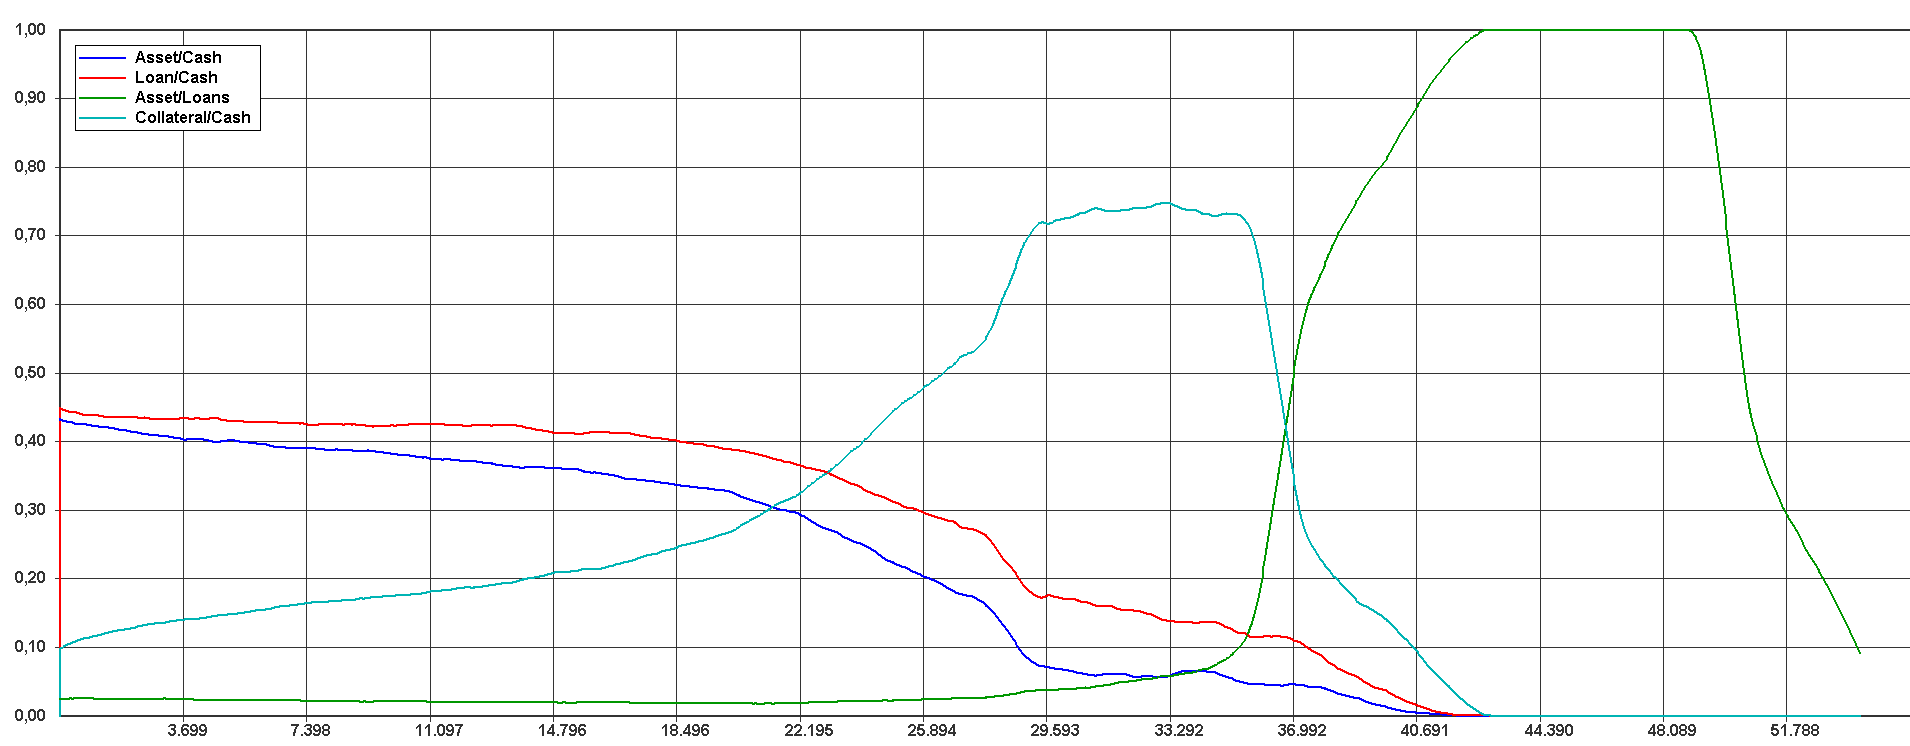
\includegraphics[width=1.0\textwidth, angle=0]{ASCENDINGCONNECTED_100_WITHCOLLATERALMARKET_MARKETSTIME_REPL.png}
	\caption{Market-activity over time of Ascending-Connected topology}
	\label{fig:wealth_ASCENDINGCONNECTED_100_WITHCOLLATERALMARKET_MARKETSTIME_REPL}
\end{figure}

\begin{figure}[H]
	\centering
  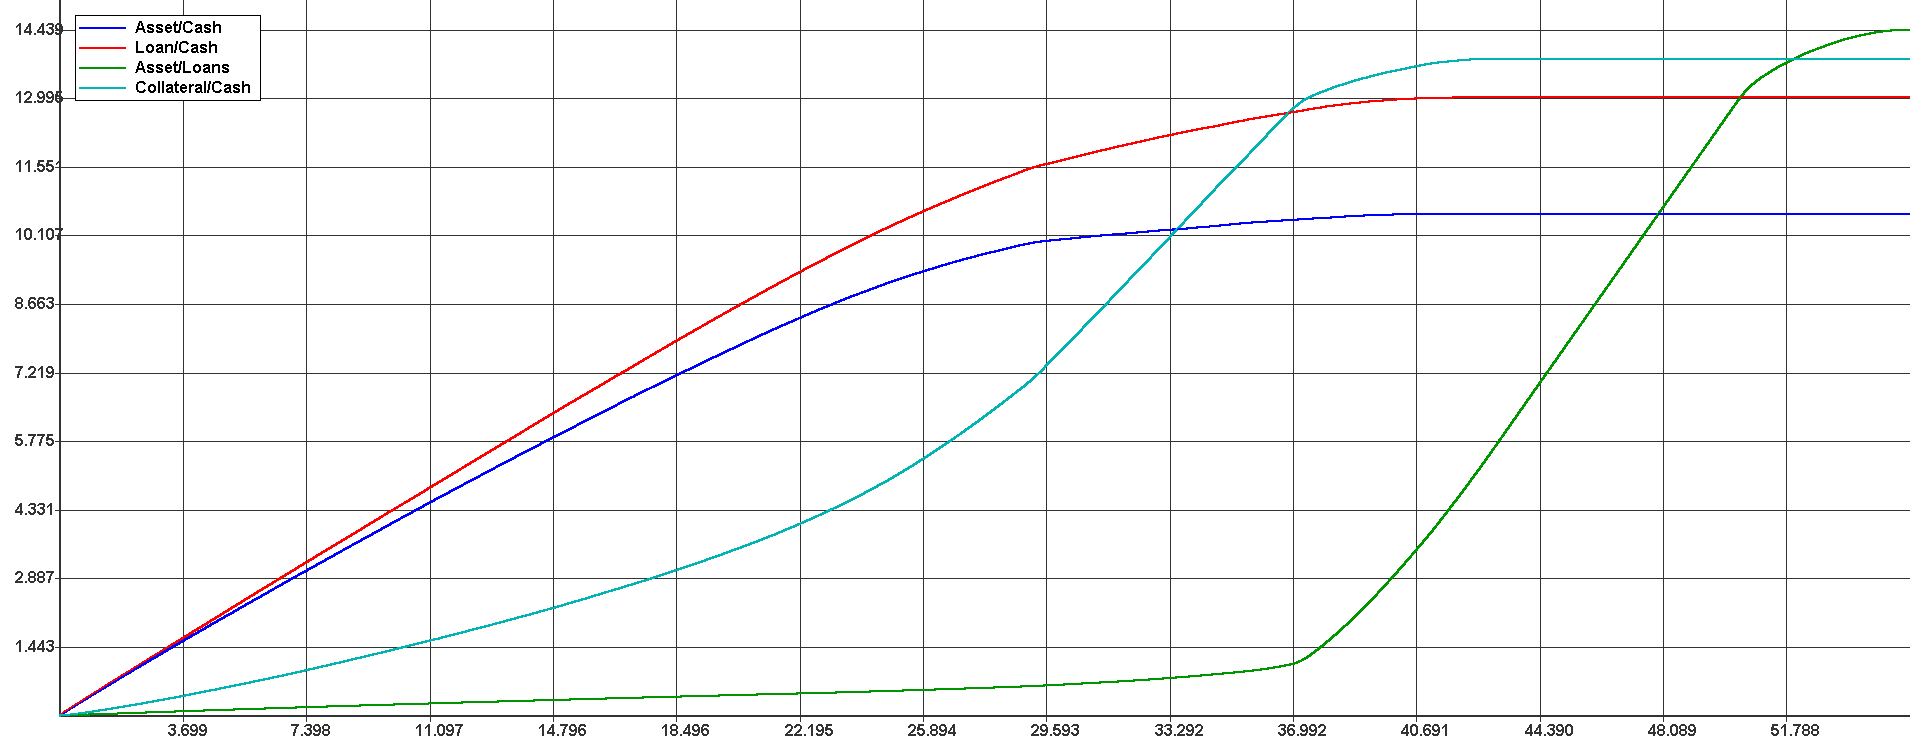
\includegraphics[width=1.0\textwidth, angle=0]{ASCENDINGCONNECTED_100_WITHCOLLATERALMARKET_MARKETSACCUM_REPL.png}
	\caption{Market-activity accumulated of Ascending-Connected topology}
	\label{fig:wealth_ASCENDINGCONNECTED_100_WITHCOLLATERALMARKET_MARKETSACCUM_REPL}
\end{figure}

\end{document}
